\documentclass[10pt]{article}
\usepackage[letterpaper,margin=0.7in]{geometry}
\usepackage{amsmath,amssymb,mathtools,booktabs,tabularx,array}
\usepackage{enumitem,xcolor,tikz,graphicx,float}
\usetikzlibrary{arrows.meta,positioning}
\usepackage[hidelinks]{hyperref}
\usepackage[font=small,labelfont=bf,skip=4pt]{caption}
\usepackage[round]{natbib}
\usepackage{titlesec}
\setlist{nosep,leftmargin=*,topsep=3pt,itemsep=2pt}
\titlespacing*{\section}{0pt}{9pt}{5pt}
\titlespacing*{\subsection}{0pt}{7pt}{3pt}
\setlength{\parindent}{0pt}
\setlength{\parskip}{4pt}
\setlength{\textfloatsep}{8pt}
\setlength{\intextsep}{7pt}
\setlength{\tabcolsep}{5pt}
\renewcommand{\arraystretch}{1.1}
\setlength{\emergencystretch}{1em}
\captionsetup{hypcap=false}
\raggedbottom
\newcommand{\I}{\mathcal{I}}
\newcommand{\V}{\mathcal{V}}
\newcommand{\E}{\mathcal{E}}
\newcommand{\C}{\mathcal{C}}
\newcommand{\K}{\mathcal{K}}
\newcommand{\Z}{\mathbb{Z}}
\newcommand{\1}{\mathbf{1}}
\newcommand{\B}{\mathsf{B}}
\newcommand{\Rd}{\mathsf{R}}
\newcommand{\As}{\mathrm{A}}
\newcommand{\Pt}{\mathrm{P}}
\begin{document}
\setlength{\abovedisplayskip}{6pt}
\setlength{\belowdisplayskip}{6pt}
\setlength{\abovedisplayshortskip}{3pt}
\setlength{\belowdisplayshortskip}{3pt}
\begin{center}
{\Large\bfseries Gray-Zone Maritime Control in the First Island Chain}\par
{\large A Networked Escalation Game}\par
Workshop 1 Report (Deliverable 2)\par
Sean Bowman, Tate Murphy, Matthew Newell\par
{\small 6.S974/2.S988/1.S980 Games, Learning, and Security, Fall 2026}
\end{center}

\section{Setting and research questions}
China and the United States compete over maritime presence and access in the First Island Chain,
including the Senkakus, Taiwan Strait, Luzon Strait, Scarborough and Second Thomas Shoals, and Paracels,
below the threshold of war. China presses its maritime claims through persistent coast-guard and militia
presence backed by PLAN ships; U.S. presence and freedom-of-navigation operations contest excessive
maritime claims and support access \citep{helmus2024,green2017}. The model represents Blue with destroyers
(DDG) and Red with navy (PLAN) and coast-guard/militia (CCG) hulls; LCS are not a separate modeled type.
Every two days, each side chooses where to station ships and whether to patrol (P) or assert (A).
Assertion abstracts actions such as shadowing, close maneuvering, querying and warning, and U.S.
freedom-of-navigation operations; it is not an identical real-world tactic for both sides.

Strategic interaction is central: control depends on the local force ratio, incidents depend on both sides'
presence and posture, war costs both players, and each side has incomplete observations of the opposing fleet.

\begin{enumerate}[label=\textbf{RQ\arabic*.}]
\item \textbf{Control and escalation.} How do incident-risk budgets affect control and war probability,
and which budget pairs are Nash equilibria in the restricted budget-choice game?
\item \textbf{Policy performance.} How do policies derived from game-theoretic models compare with
random and rule-based policies in payoff, control, and war probability against a common set of opponents?
\item \textbf{Robustness and redesign.} Do the best Blue policies and designs under nominal weather
also perform best in expected and worst-case payoff across weather scenarios, against the tested Red policies?
\end{enumerate}
Outcomes are estimated over 200 seeds per configuration: each player's payoff, the fraction of games ending
in war, and Blue's average value-weighted control index
$\bar c_\B=\tau^{-1}\sum_{t=1}^{\tau}(\sum_v V_v^\B c_v^{t+1})/(\sum_v V_v^\B)\in[-1,1]$.
RQ3 also compares scenario-weighted and worst-scenario payoff. Repeated-game restraint is a supporting
analytical example, rather than a separate simulation claim.

\textbf{Response to proposal feedback.}
\begin{center}\small
\begin{tabularx}{\textwidth}{@{}p{0.29\textwidth}X@{}}
\toprule
Feedback & Revision\\\midrule
Make the model explicit & Define state, actions, observations, transitions and payoffs (\S3).\\
Formulate Q1 as a MIP & Use a myopic allocation MIP; risk budgets replace informal player types (\S3.4).\\
Deepen the research questions & Add a budget-choice game, policy comparisons, and resilience analysis (\S4).\\
Specify uncertainty and redesign & Four weather scenarios and three Blue designs address the robustness feedback (\S3).\\
Supply parameters and evidence & Mark parameter values as assumptions; report analytical results and 77 configurations with 200 seeds each (\S4).\\
\bottomrule
\end{tabularx}
\end{center}

\section{Literature and current practice}
\citet{helmus2024} document Chinese gray-zone tactics, including persistent presence, resupply obstruction
and water cannon; \citet{green2017} discuss deterrence and escalation management. CUES provides an encounter-management
reference \citep{cues2014}. These motivate the action categories and asymmetric hull types, rather than calibrating numerical parameters.

The model combines structured gray-zone gaming \citep{wasser2019}, game-based patrol allocation
\citep{shieh2012}, network interdiction \citep{washburn1995}, and escalation through shared risk
\citep{schelling1966}. Its contribution is a computable general-sum game for comparing policies and designs.
Control, incident hazards and weather probabilities are modeling assumptions, not empirical estimates.

\newpage
\section{Game formulation}
\subsection{Agents, network and state}
Players are $\I=\{\B,\Rd\}$: Blue has 10 DDG; Red has 8 PLAN and 6 CCG hulls.
The undirected graph $G=(\V,\E)$ contains home ports $H_\B=\{\mathrm{YOK,GUA}\}$,
$H_\Rd=\{\mathrm{NBO,SAN}\}$ and eight contested zones $\C$ (Fig.~\ref{fig:net}).
One period is two days; moving one edge takes one period.

\begin{figure}[H]\centering
\begin{minipage}{0.36\textwidth}\centering
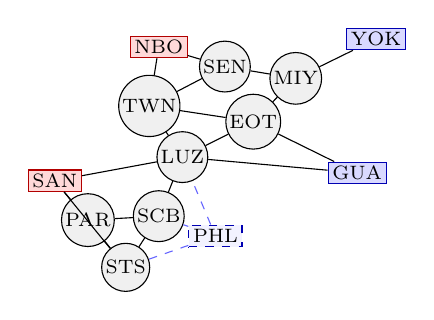
\begin{tikzpicture}[x=0.12cm,y=0.10cm,
  c/.style={circle,draw,fill=gray!12,inner sep=0.8pt,font=\scriptsize},
  hb/.style={rectangle,draw=blue!70!black,fill=blue!15,inner sep=1.5pt,font=\scriptsize},
  hr/.style={rectangle,draw=red!70!black,fill=red!15,inner sep=1.5pt,font=\scriptsize},
  hd/.style={rectangle,draw=blue!70!black,dashed,fill=blue!5,inner sep=1.5pt,font=\scriptsize}]
\node[hr] (NBO) at (10,25) {NBO}; \node[c] (SEN) at (17,22.5) {SEN}; \node[c] (MIY) at (24.5,21) {MIY};
\node[hb] (YOK) at (33,26) {YOK}; \node[c] (TWN) at (9,17.5) {TWN}; \node[c] (EOT) at (20,15.5) {EOT};
\node[c] (LUZ) at (12.5,11) {LUZ}; \node[hb] (GUA) at (31,9) {GUA}; \node[hr] (SAN) at (-1,8) {SAN};
\node[c] (PAR) at (2.5,3) {PAR}; \node[c] (SCB) at (10,3.5) {SCB}; \node[c] (STS) at (6.5,-3) {STS};
\node[hd] (PHL) at (16,1) {PHL};
\foreach \a/\b in {YOK/MIY,MIY/SEN,MIY/EOT,SEN/NBO,SEN/TWN,NBO/TWN,TWN/EOT,TWN/LUZ,
  EOT/LUZ,EOT/GUA,GUA/LUZ,LUZ/SCB,LUZ/SAN,SCB/STS,SCB/PAR,PAR/SAN,SAN/STS,STS/PAR}
  \draw (\a)--(\b);
\foreach \a/\b in {PHL/SCB,PHL/LUZ,PHL/STS} \draw[dashed,blue!60] (\a)--(\b);
\end{tikzpicture}
\end{minipage}\hfill
\begin{minipage}{0.61\textwidth}\small
\textbf{Sequence within each period}
\begin{enumerate}
\item Nature updates regional weather; players receive observations.
\item Endurance rules identify ships that must return or refit.
\item Both sides choose moves and postures simultaneously.
\item Moves resolve within fleet movement budgets; endurance updates.
\item Control and incidents update; escalation rises or falls.
\item Payoffs accrue; play stops at war or after 60 periods.
\end{enumerate}
\end{minipage}
\caption{Network and sequence of play. Squares are ports; circles are contested zones.
Dashed links and PHL are the additional access assumed in design D1.}
\label{fig:net}
\end{figure}

The state is $s^t=(x^t,d^t,c^t,\ell^t,w^t)$:
\begin{center}\small
\begin{tabularx}{\textwidth}{@{}lXlX@{}}
\toprule
Symbol & Meaning & Symbol & Meaning\\\midrule
$x^t_{k,v}$ & Type-$k$ ship count at node $v$ & $d^t_s$ & Ship $s$'s remaining endurance\\
$c^t_v$ & Control: $-1$ Red to $+1$ Blue & $\ell^t$ & Escalation: $0$ to $L=5$ (war)\\
$w^t_r$ & Calm, rough or storm in region $r$ & $V_v^i$ & Player $i$'s value for zone $v$\\
\bottomrule
\end{tabularx}
\end{center}

\subsection{Actions, constraints, information and uncertainty}
Each free ship stays or moves to an adjacent legal node; each occupied zone receives posture
$p_{i,v}\in\{\Pt,\As\}$. For directed traversals $(u,v)$ of the undirected edges, let
$f^t_{k,uv}\in\Z_{\ge0}$ count moving ships. For $k\in\K_i$,
\begin{align*}
x^{t+1}_{k,u}&=x^t_{k,u}+\sum_{v\in\delta(u)}f^t_{k,vu}-\sum_{v\in\delta(u)}f^t_{k,uv}
&&\text{(ship conservation)},\\
\sum_{v\in\delta(u)}f^t_{k,uv}&\le x^t_{k,u},\qquad
\sum_{k\in\K_i,(u,v)}f^t_{k,uv}\le F_i
&&\text{(available ships; movement cap)}.
\end{align*}
Here $\delta(u)$ denotes adjacent nodes and $F_\B=8$, $F_\Rd=10$ ship movements per period.
This is a logistical movement proxy, not a fuel inventory. Ships with $d_s\le\operatorname{dist}(v,H_i)$
receive return priority; one full period in port resets endurance to $D_k$. Opponent ports and storm-closed
nodes cannot be entered; ships in storm zones hold. The engine executes return moves first up to $F_i$;
unexecuted moves hold, and free ships use the remaining budget.

\textbf{Information.} Each side sees its own fleet and public control, escalation and weather.
At each observed node it draws a Bernoulli detection with probability $q_{i,v}$: $0.95$ with a ship present,
$0.6$ with an adjacent ship or own-port coverage, and $0.2$ otherwise. Red has a $0.6$ floor at four coastal
zones before the bad-weather multiplier $0.7$. Conditional on the state, detections are drawn independently.
Success reveals exact counts by type and posture; a miss retains the last observation. Initial counts are
known. This is a last-seen estimate, not a Bayesian belief distribution.

\textbf{Weather.} Scenarios $\omega=(\text{calm, nominal, typhoon, extreme})$ have weights
$\pi=(0.25,0.40,0.25,0.10)$. Regional three-period storms start with probabilities
$p_s=(0,0.02,0.06,0.12)$ when no storm is active; otherwise rough-sea probabilities are
$p_r=(0,0.2,0.35,0.5)$. Storms freeze local control and prevent incidents; rough seas halve CCG effectiveness.

\subsection{Transitions and payoffs}
Local strength and control respond to presence and posture:
\begin{equation}
S_{i,v}=\sum_{k\in\K_i}w_k\alpha^{\1[p_{i,v}=\As]}x_{k,v},\quad
\phi_v=\frac{S_{\B,v}-S_{\Rd,v}}{S_{\B,v}+S_{\Rd,v}+\kappa},\quad
c^{t+1}_v=(1-\lambda)c^t_v+\lambda\phi_v.\label{eq:control}
\end{equation}
Strength uses post-move counts. Here $w_{\rm DDG}=w_{\rm PLAN}=1$, $w_{\rm CCG}=0.6$
($0.3$ in rough seas), $\alpha=1.5$, $\lambda=0.3$, and $\kappa=1$.

\newpage
\textbf{Incidents and escalation.} At a non-storm zone, an incident has probability $\rho_v=1-e^{-h_v}$,
\begin{equation}
h_v=\big(h_0+h^\B_\As\1[p_{\B,v}=\As]+h^\Rd_\As\1[p_{\Rd,v}=\As]\big)
\min\{S_{\B,v},S_{\Rd,v}\}(1+\ell^t/2).\label{eq:hazard}
\end{equation}
Red's assertion coefficient is weighted by its PLAN/CCG strength mix. Each incident raises escalation by
one, capped at $L$; with no incidents, escalation falls by one with probability $\mu$ (floor zero).

\textbf{Payoffs.} Let $m_i^t$ count executed moves, $\sigma_\B=1$, $\sigma_\Rd=-1$, and $C_i$
be the per-period design cost ($C_\Rd=0$). If $\ell^{t+1}$ is the post-turn escalation,
\begin{equation}
g_i^t=\sigma_i\sum_{v\in\C}V_v^i c_v^{t+1}-\gamma m_i^t-\eta\ell^{t+1}-C_i,
\qquad u_i=\sum_{t=1}^{\tau}\delta^{t-1}g_i^t-W\1[\text{war}].\label{eq:payoff}
\end{equation}
The horizon $\tau$ is the earlier of $T=60$ and the first turn ending at $\ell=L$.
Different zone values and a shared war cost make this a general-sum game.

\begin{table}[H]\centering\small
\begin{tabular}{@{}lrrrrrrrr@{}}
\toprule
Zone & TWN & SEN & MIY & EOT & LUZ & SCB & STS & PAR\\\midrule
$V_v^\B$ &10&6&4&4&6&5&5&2\\
$V_v^\Rd$ &10&6&3&4&5&7&6&6\\
$c_v^1$ &0&0.2&0.3&0.2&0.1&$-0.2$&0&$-0.4$\\\bottomrule
\end{tabular}
\caption{Assumed zone values and initial control.}\label{tab:params}
\end{table}
\begin{center}\small
\begin{tabularx}{\textwidth}{@{}lX@{}}
\toprule
Parameter group & Assumed values\\\midrule
Payoff and escalation & $\delta=0.98$, $\gamma=0.1$, $\eta=1$, $W=200$, $\ell^1=1$, $\mu=0.25$\\
Incident hazard & $h_0=0.006$; assertion: Blue $0.03$, Red PLAN $0.036$, CCG $0.012$\\
Endurance and incident cost & $D_{\rm DDG}=10$, $D_{\rm PLAN}=8$, $D_{\rm CCG}=6$ periods; $\Lambda=20$\\
\bottomrule
\end{tabularx}
\end{center}

\subsection{Decision models: myopic allocation and template game}\label{sec:mip}
The \emph{MIP-BR} policy optimizes a myopic surrogate against last-seen counts and postures, rather than
the full dynamic game. Let $y_{s,w}$ select a legal destination
$w\in A_s$ for free ship $s$, and let $b_{v,(n,p)}$ select a count vector $n$ and posture $p$ at zone $v$.
Tabulating $\phi_v(n,p)$ and $\rho_v(n,p)$ makes the allocation problem linear:
\begin{align*}
\max_{y,b,z}\quad &\textstyle\sum_{v\in\C,(n,p)}a_v(n,p)b_{v,(n,p)}
-\gamma\textstyle\sum_{s,w\ne\mathrm{loc}(s)}y_{s,w}-1000z\\
\text{s.t.}\quad &\textstyle\sum_{w\in A_s}y_{s,w}=1 &&\forall s\quad\text{(one destination)},\\
&\textstyle\sum_{s,w\ne\mathrm{loc}(s)}y_{s,w}\le F_i^{\rm rem}&&\text{(remaining movement budget)},\\
&\textstyle\sum_{(n,p)}b_{v,(n,p)}=1&&\forall v\quad\text{(one zone option)},\\
&\textstyle\sum_{(n,p)}n_k b_{v,(n,p)}=\bar x_{k,v}+\textstyle\sum_{s:\,k(s)=k}y_{s,v}
&&\forall v,k\quad\text{(consistent counts)},\\
&\textstyle\sum_{v,(n,p)}\rho_v(n,p)b_{v,(n,p)}\le\varepsilon_i(1-\ell^t/L)+z
&&\text{(incident-risk allowance)},\\
&y,b\in\{0,1\},\quad z\ge0.&&
\end{align*}
Here $a_v=V_v^i\lambda H\sigma_i\phi_v-\Lambda\rho_v$, $H=[1-\delta(1-\lambda)]^{-1}$ weights control persistence,
$\bar x$ counts prescribed return/refit positions, and
$F_i^{\rm rem}=\max(0,F_i-\text{prescribed return moves})$. Variables for illegal destinations are absent.
The risk sum estimates \emph{expected incidents this turn}, not war probability.
Penalized slack $z$ makes the budget soft. Budgets $\varepsilon_i\in\{0.05,0.15,0.40\}$ represent
conservative, moderate and aggressive play.

\textbf{Template game.} Each player chooses one of 14 templates: seven regional fleet splits times two
postures. With calm weather and $\ell=1$, payoffs are
$M_i=\sigma_i\sum_v V_v^i\phi_v-\Lambda\sum_v\rho_v$.
Dominance, Nash equilibria, maximin and correlated-equilibrium LPs apply to this restricted game $\Gamma$.
Its equilibrium and maximin policies are then tested in the simulator, alongside random, rule-based,
greedy and MIP-BR policies. Equilibrium guarantees do not transfer automatically to the simulator.

\subsection{Blue redesigns}\label{sec:designs}
\textbf{D1: dispersed basing} adds an assumed PHL port and links to SCB/LUZ/STS (cost $0.3$/period).
\textbf{D2: sensing} adds a $0.6$ detection floor in contested zones, including bad weather (cost $0.5$/period).
\textbf{D3: hotline} raises $\mu$ to $0.5$ and halves assertion hazards when $\ell\ge3$ (zero assumed cost).
Two unitary actors, last-seen estimates and myopic decisions remain limitations.

\newpage
\section{Preliminary results}
\S4.1--4.2 are analytical (template game); the rest use 200 seeds per configuration, the same for every policy.
Unless stated, Red plays MIP-BR with $\varepsilon_\Rd=0.15$ in nominal weather.

\subsection{Small example: patrol or assert, and sustainable restraint}
Fix the force splits that survive dominance (\S4.2): Blue center-heavy, Red south-heavy. Each side then only
chooses P or A. The resulting $2\times2$ sub-matrix of $\Gamma$, normalized so (P,P) $=(0,0)$, has
(P,A) $=(-9.61,\,1.20)$, (A,P) $=(0.28,\,-10.45)$ and (A,A) $=(-11.41,\,-11.33)$ (Blue, Red).
Asserting against a patroller pays a little (one-period gain $G_\B=0.28$, $G_\Rd=1.20$), but mutual assertion costs more than
patrolling alone, so $BR_i(\Pt)=\As$ and $BR_i(\As)=\Pt$: the same structure as the
shared-compute example (Lecture 3). There are two pure NE, (A,P) and (P,A), and a mixed NE (Blue asserts w.p.\
$0.58$, Red $0.13$) with mutual assertion w.p.\ $0.08$ and payoffs $v_\B=-1.25$, $v_\Rd=-6.06$. The welfare-maximizing correlated equilibrium (CE LP)
puts $0.40$ on (P,P), $0.54$ on (A,P), $0.06$ on (P,A) and \emph{zero} on (A,A): a mediator (e.g.\ a hotline)
removes mutual assertion.

In the repeated game (Lectures 5--6), consider grim trigger: both patrol; after any assertion, both play the
mixed NE forever. By the one-stage deviation principle, patrolling is optimal iff
$(1-\delta)G_i+\delta v_i\le0$, i.e.\ $\delta\ge G_i/(G_i-v_i)$, which is $0.18$ for Blue and $0.17$ for Red. With
$\delta=0.98$, \textbf{mutual restraint is a subgame perfect equilibrium}, although our one-period-ahead policies
cannot see this yet.

\subsection{Template game: dominance, equilibria and the effect of the escalation cost}
IESDS reduces $\Gamma$ from $14\times14$ to $2\times4$: Blue keeps only the center-heavy split (20\% North, 60\% Center, 20\% South),
Red the south- or center/south-heavy splits. There are two pure NE: (Blue C-heavy assert, Red S-heavy patrol),
payoffs $(0.39,-9.27)$, and (Blue C-heavy patrol, Red C/S assert), $(-14.44,2.71)$; the \emph{equilibrium} policy
plays the first (higher total payoff; this selection is an assumption). Without the escalation cost, the zero-sum
maximin LP has a pure equilibrium where \emph{both} sides concentrate on the Center and assert (value $-2.26$):
the shared incident cost is what makes at most one side assert.

\subsection{RQ1: control versus war risk, and the risk-budget game}
\begin{figure}[!ht]
\centering
\begin{minipage}{0.40\textwidth}\centering
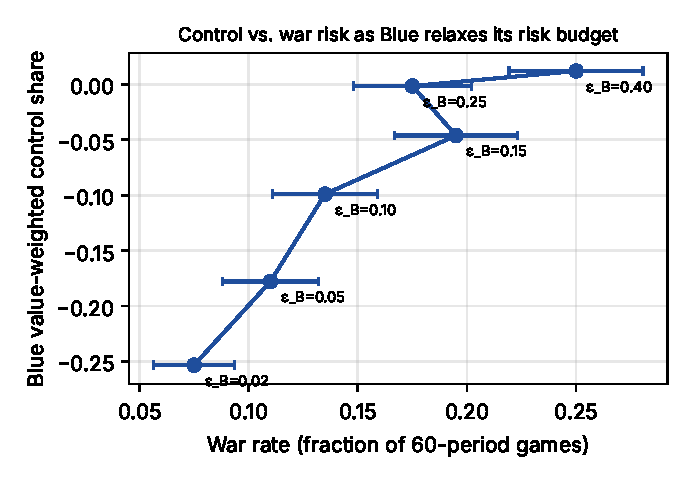
\includegraphics[width=\textwidth,height=3.7cm,keepaspectratio]{figures/frontier.pdf}
\end{minipage}\hfill
\begin{minipage}{0.54\textwidth}\centering\small
\begin{tabular}{l|ccc}
\toprule
$\B\backslash\Rd$ & cons.\ $0.05$ & mod.\ $0.15$ & aggr.\ $0.40$\\\midrule
cons.\ $0.05$ & $-194,\ 199$ & $-303,\ 315$ & $-308,\ 318$\\
              & war $0.10$ & $0.11$ & $0.12$\\
mod.\ $0.15$  & $18,\ -36$ & $-144,\ 101$ & $-192,\ 140$\\
              & war $0.15$ & $0.20$ & $0.21$\\
aggr.\ $0.40$ & $74,\ -80$ & $-83,\ 16$ & $\mathbf{-151,\ 39}$\\
              & war $0.14$ & $0.25$ & $\mathbf{0.34}$\\
\bottomrule
\end{tabular}
\end{minipage}
\caption{Left: Blue's control share vs.\ war rate as Blue's risk budget $\varepsilon_\B$ grows (Red fixed at $0.15$).
Right: the risk-budget game, $(u_\B,u_\Rd)$ and war rate when both sides choose $\varepsilon$ (s.e.\ $\approx 5$--$12$).
Bold: the unique Nash equilibrium.}
\label{fig:rq1}
\end{figure}
\textbf{Frontier.} Raising $\varepsilon_\B$ from $0.02$ to $0.15$ lifts Blue's control share from $-0.25$ to
$-0.05$ while the war rate rises from $0.07$ to $0.20$; going to $0.40$ adds only $0.06$ of control
(Fig.~\ref{fig:rq1}). Most of what a looser budget buys is bought by $\varepsilon\approx0.15$--$0.25$.

\textbf{Risk-budget game.} When both sides pick a budget, ``aggressive'' is a best response to every opponent
choice for both players (Red vs.\ conservative Blue, $318$ vs.\ $315$, is within noise), so (aggressive,
aggressive) is the unique pure NE. It has the \emph{highest} war rate ($0.34$ vs.\ $0.10$ when both are
conservative) and total payoff $-112$ vs.\ $+12$ at (conservative, moderate): a prisoner's dilemma (Lecture 3).
So restraint must come from repetition or coordination (\S4.1).

\subsection{RQ2: strategic versus heuristic play}
\begin{table}[!ht]\centering\small
\begin{tabular}{l|ccc|c}
\toprule
Blue $\backslash$ Red & rule-based (moderate) & MIP-BR & equilibrium & worst case over Red\\\midrule
random & $-283$ / $-0.14$ / $0.15$ & $-319$ / $-0.16$ / $0.33$ & $-164$ / $-0.08$ / $0.06$ & $-319$\\
rule-based (moderate) & $-122$ / $-0.05$ / $0.04$ & $-184$ / $-0.09$ / $0.06$ & $35$ / $+0.06$ / $0.04$ & $-184$\\
greedy & $-70$ / $+0.01$ / $0.12$ & $-137$ / $-0.05$ / $0.14$ & $65$ / $+0.08$ / $0.03$ & $-137$\\
MIP-BR & $-75$ / $+0.01$ / $0.13$ & $-144$ / $-0.05$ / $0.20$ & $53$ / $+0.08$ / $0.08$ & $-144$\\
equilibrium & $-72$ / $-0.01$ / $0.07$ & $\mathbf{-116}$ / $-0.03$ / $0.10$ & $21$ / $+0.05$ / $0.06$ & $\mathbf{-116}$\\
maximin & $-170$ / $-0.09$ / $0.04$ & $-221$ / $-0.12$ / $0.08$ & $-35$ / $-0.01$ / $0.00$ & $-221$\\
\bottomrule
\end{tabular}
\caption{Blue payoff $u_\B$ / control share / war rate (s.e.\ of $u_\B$ is 1--7). Nominal weather, design D0.}
\label{tab:policies}
\end{table}
Greedy, MIP-BR and equilibrium beat the random and rule-based benchmarks (Table~\ref{tab:policies}). The
\textbf{equilibrium} policy has the best worst case over Red's policies ($-116$) and, against MIP-BR, half the war
rate of MIP-BR itself ($0.10$ vs.\ $0.20$). Greedy and MIP-BR do best against weaker opponents but escalate more.
\textbf{Maximin} is the safest (war rate $\le0.08$) but gives up the most control: it guards against a worst-case
Red template that Red rarely plays.

\textbf{MIP vs.\ greedy.} Over 1{,}524 Blue decisions in 30 games the greedy heuristic matched the MIP optimum
in 67\% of decisions but broke the risk budget in 14\%, so the MIP is needed to enforce the feasible region
exactly; in play the two perform about the same.

\subsection{RQ3: robustness to weather and resilient designs}
\subsection{RQ3: weather robustness and resilient designs}
For policy or design $x$, let $J(x,\omega)$ be its simulated mean payoff under scenario $\omega$.
We compare $\sum_\omega\pi_\omega J(x,\omega)$ and $\min_\omega J(x,\omega)$.
The latter is the worst scenario mean, not the worst individual run or worst possible opponent.
\begin{figure}[H]\centering
\begin{minipage}{0.35\textwidth}\centering
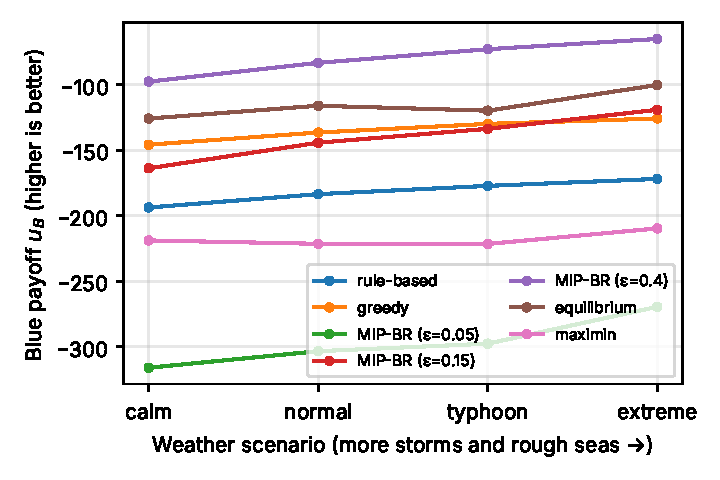
\includegraphics[width=\textwidth]{figures/weather.pdf}
\end{minipage}\hfill
\begin{minipage}{0.63\textwidth}\centering\small
\setlength{\tabcolsep}{3pt}
\begin{tabular}{@{}lrrrrrr@{}}\toprule
Design & Calm & Nom. & Typh. & Extr. & Exp. & Worst\\\midrule
D0 & $-164$ & $-144$ & $-134$ & $-119$ & $-144$ & $-164$\\
D1 & $-153$ & $-141$ & $-131$ & $\mathbf{-98}$ & $-137$ & $-153$\\
D2 & $-181$ & $-164$ & $-149$ & $-136$ & $-162$ & $-181$\\
D3 & $\mathbf{-140}$ & $\mathbf{-118}$ & $\mathbf{-111}$ & $-102$ & $\mathbf{-120}$ & $\mathbf{-140}$\\\bottomrule
\end{tabular}
\end{minipage}
\caption{Left: Blue policy payoffs by weather. Right: Blue design payoffs with MIP-BR on both sides
(reported s.e.\ approximately 7); D0 baseline, D1 basing, D2 sensing, D3 hotline.}\label{fig:rq3}
\end{figure}
\textbf{Weather.} Most tested policies do worst in calm seas: rough seas weaken Red's CCG hulls and storms
pause incidents. Baseline MIP-BR's war rate falls from $0.24$ (calm) to $0.10$ (extreme). MIP-BR with
$\varepsilon_\B=0.40$ and the equilibrium-derived policy rank first and second in all four scenarios.
The highest-payoff policy also has war rates of $0.12$--$0.29$, making sensitivity to $W=200$ important.

\textbf{Designs.} D3 has the best expected and worst-scenario payoff; in nominal weather it cuts war rate
from $0.20$ to $0.05$ and increases Red's payoff from $101$ to $144$. Its zero cost is an assumption.
D1 barely changes Blue's nominal payoff, reduces Red's from $101$ to $16$, and raises war rate to $0.28$.
D2 shows no measurable benefit even in the reported zero-cost check. Red recomputes actions under its
fixed MIP-BR policy; these experiments do not re-solve equilibrium policy selection after redesign.

\textbf{Limits of inference.} Numerical values are assumptions. The findings are comparisons within the model,
not calibrated forecasts of conflict. War rates depend on hazards, de-escalation and war penalties.
Small payoff gaps should be treated cautiously given Monte Carlo error; formal comparisons require
uncertainty estimates for payoff differences. The engine's return-move cap can also make executed positions
differ from the MIP's prescribed fixed positions when returns alone exceed the cap.


\textbf{Limitations.} Parameters are assumptions; policies look one period ahead; the war rate depends strongly on
$h$, $\mu$ and $W$; payoff differences below about 20 are ties (s.e.\ 5--12).

\newpage
\subsection{RQ3: weather robustness and resilient designs}
For policy or design $x$, let $J(x,\omega)$ be its simulated mean payoff under scenario $\omega$.
We compare $\sum_\omega\pi_\omega J(x,\omega)$ and $\min_\omega J(x,\omega)$.
The latter is the worst scenario mean, not the worst individual run or worst possible opponent.
\begin{figure}[H]\centering
\begin{minipage}{0.35\textwidth}\centering
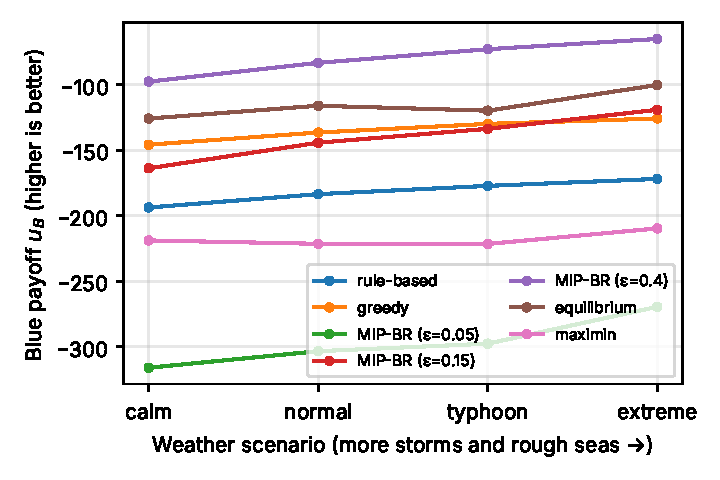
\includegraphics[width=\textwidth]{figures/weather.pdf}
\end{minipage}\hfill
\begin{minipage}{0.63\textwidth}\centering\small
\setlength{\tabcolsep}{3pt}
\begin{tabular}{@{}lrrrrrr@{}}\toprule
Design & Calm & Nom. & Typh. & Extr. & Exp. & Worst\\\midrule
D0 & $-164$ & $-144$ & $-134$ & $-119$ & $-144$ & $-164$\\
D1 & $-153$ & $-141$ & $-131$ & $\mathbf{-98}$ & $-137$ & $-153$\\
D2 & $-181$ & $-164$ & $-149$ & $-136$ & $-162$ & $-181$\\
D3 & $\mathbf{-140}$ & $\mathbf{-118}$ & $\mathbf{-111}$ & $-102$ & $\mathbf{-120}$ & $\mathbf{-140}$\\\bottomrule
\end{tabular}
\end{minipage}
\caption{Left: Blue policy payoffs by weather. Right: Blue design payoffs with MIP-BR on both sides
(reported s.e.\ approximately 7); D0 baseline, D1 basing, D2 sensing, D3 hotline.}\label{fig:rq3}
\end{figure}
\textbf{Weather.} Most tested policies do worst in calm seas: rough seas weaken Red's CCG hulls and storms
pause incidents. Baseline MIP-BR's war rate falls from $0.24$ (calm) to $0.10$ (extreme). MIP-BR with
$\varepsilon_\B=0.40$ and the equilibrium-derived policy rank first and second in all four scenarios.
The highest-payoff policy also has war rates of $0.12$--$0.29$, making sensitivity to $W=200$ important.

\textbf{Designs.} D3 has the best expected and worst-scenario payoff; in nominal weather it cuts war rate
from $0.20$ to $0.05$ and increases Red's payoff from $101$ to $144$. Its zero cost is an assumption.
D1 barely changes Blue's nominal payoff, reduces Red's from $101$ to $16$, and raises war rate to $0.28$.
D2 shows no measurable benefit even in the reported zero-cost check. Red recomputes actions under its
fixed MIP-BR policy; these experiments do not re-solve equilibrium policy selection after redesign.

\textbf{Limits of inference.} Numerical values are assumptions. The findings are comparisons within the model,
not calibrated forecasts of conflict. War rates depend on hazards, de-escalation and war penalties.
Small payoff gaps should be treated cautiously given Monte Carlo error; formal comparisons require
uncertainty estimates for payoff differences. The engine's return-move cap can also make executed positions
differ from the MIP's prescribed fixed positions when returns alone exceed the cap.

\section{Prototype}
% !TEX root = report.tex
\noindent\begin{minipage}[t]{0.56\textwidth}\vspace{0pt}
\textbf{Current state:} \texttt{wargame\_gui.py} runs the model of \S3 as a \textbf{GUI} (Fig.~\ref{fig:gui}: pick
each side's plan, Blue's design and the weather, then step through turns or run many games; a Help button explains
the map), as \textbf{batch} runs, or as a turn-by-turn \textbf{trace}. \texttt{experiments.py all} regenerates
every number in \S4; instructions are in \texttt{README.md}.

\smallskip\noindent \textbf{How the code reflects the model:} \texttt{Game.step} is the timeline of Fig.~\ref{fig:net} with
\eqref{eq:control}--\eqref{eq:payoff}; \texttt{MIPBRPolicy} solves the MIP of \S\ref{sec:mip} each period;
\texttt{MetaGame} builds $\Gamma$ and runs IESDS, NE enumeration and both LPs.

\smallskip\noindent 
\textbf{Still to build:} Learning agents, an attacker that reacts to Blue, Bayesian beliefs and multi-period
policies (\S6).
\end{minipage}\hfill
\begin{minipage}[t]{0.41\textwidth}\vspace{0pt}\centering
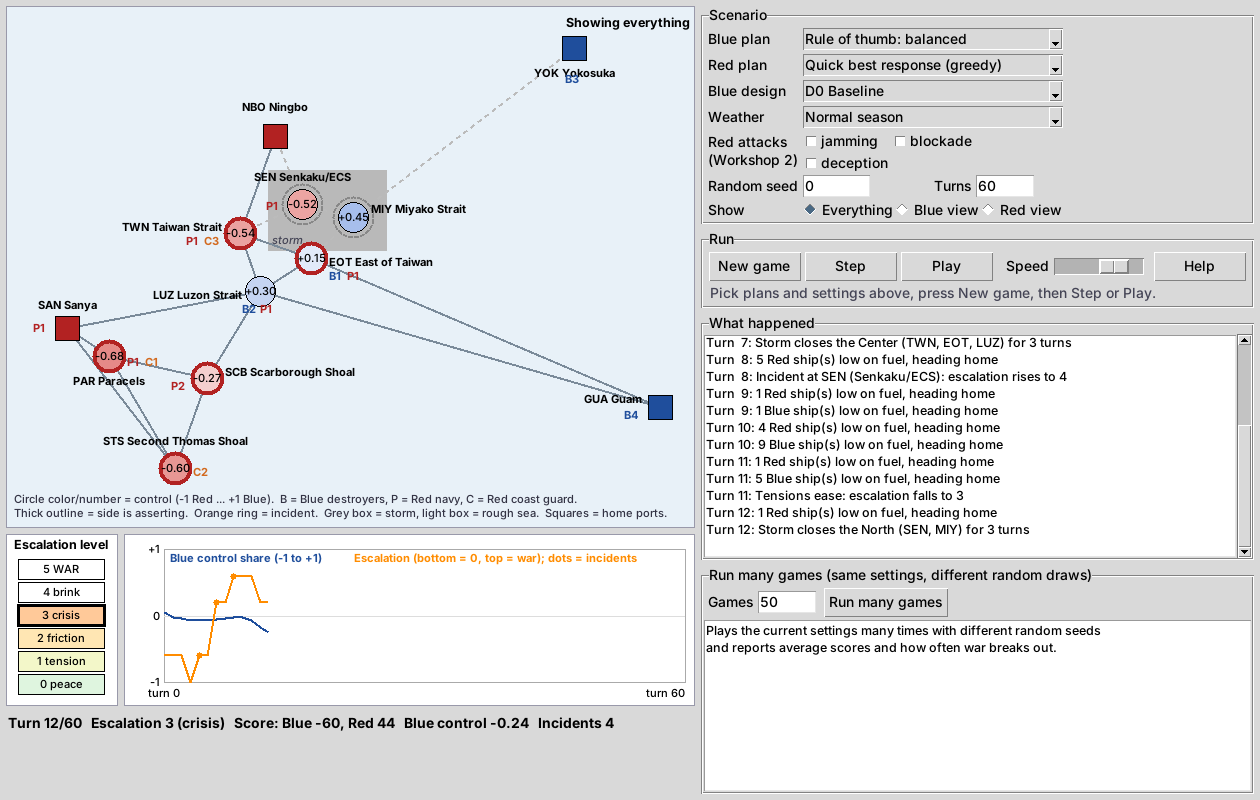
\includegraphics[width=\textwidth]{figures/gui_screenshot.png}
\captionof{figure}{The GUI after 12 turns (storm in the North).}\label{fig:gui}
\end{minipage}

\section{Plan for Workshop 2}
\textbf{Model.} Bayesian beliefs (Lectures 7--8), multi-period best response, $\pm50\%$ sweep on $V,h,W,\mu$.

\textbf{Learning (Module 2, once taught).} A Red agent that learns from repeated play (reinforcement learning), and
fictitious-play or no-regret updates on the template game. Do they converge or cycle, drift toward restraint or
assertion, and exploit the predictable rule-based Blue policy?

\textbf{Attacks and defenses (Module 3).} Run the three coded Red attacks (CCG blockade of Blue's edges at SCB/STS,
jamming of Blue sensing, false contacts) and an attacker that moves after seeing Blue's posture (backward
induction). Defenses: randomized patrols, D1, D2; metric: change in control and war rate.

\textbf{Resilient designs (Module 4).} D0--D3 and combinations under attack and a rare long typhoon; price the hotline.
\textbf{Timeline:} Nov 3 beliefs, attacks; Nov 17 learning; Dec 1 redesigns; Dec 8 report.

\clearpage
\begin{thebibliography}{99}\small\setlength{\itemsep}{0pt}
\bibitem[Green et~al.(2017)]{green2017} Green, M., Hicks, K., Cooper, Z., Schaus, J., and Douglas, J. (2017).
\emph{Countering Coercion in Maritime Asia: The Theory and Practice of Gray Zone Deterrence}. Center for Strategic and International Studies.
\bibitem[Helmus et~al.(2024)]{helmus2024} Helmus, T. C., Romita Grocholski, K., Liggett, T., Rhoades, A. L., Savitz, S., and Palmer, K. (2024).
\emph{Understanding and Countering China's Maritime Gray Zone Operations} (RR-A2954-1). RAND Corporation. \url{https://doi.org/10.7249/RRA2954-1}
\bibitem[Schelling(1966)]{schelling1966} Schelling, T. C. (1966). \emph{Arms and Influence}. Yale University Press.
\bibitem[Shieh et~al.(2012)]{shieh2012} Shieh, E., An, B., Yang, R., Tambe, M., Baldwin, C., DiRenzo, J., Maule, B., and Meyer, G. (2012).
PROTECT: A deployed game theoretic system to protect the ports of the United States. In \emph{Proc.\ AAMAS 2012}, 13--20.
\bibitem[Washburn and Wood(1995)]{washburn1995} Washburn, A., and Wood, K. (1995). Two-person zero-sum games for network interdiction. \emph{Operations Research}, 43(2), 243--251.
\bibitem[Wasser et~al.(2019)]{wasser2019} Wasser, B., Oberholtzer, J., Pettyjohn, S. L., and Mackenzie, W. (2019).
\emph{Gaming Gray Zone Tactics: Design Considerations for a Structured Strategic Game} (RR-2915-A). RAND Corporation. \url{https://doi.org/10.7249/RR2915}
\bibitem[WPNS(2014)]{cues2014} Western Pacific Naval Symposium (2014). \emph{Code for Unplanned Encounters at Sea (CUES)}.
\end{thebibliography}

\end{document}
